% !TEX TS-program = xelatex
% !BIB TS-program = bibtex
\documentclass[12pt,letterpaper]{article}
\usepackage{style/dsc180reportstyle}
\usepackage{booktabs}
\usepackage{float}      % for [H] placement option
\usepackage{placeins}   % for \FloatBarrier
% import dsc180reportstyle.sty

%%%%%%%%%%%%%%%%%%%%%%%%%%%%%%%%%%%%%%%%%%%%%%%%%%%%%%%%
%%%% Title and Authors
%%%%%%%%%%%%%%%%%%%%%%%%%%%%%%%%%%%%%%%%%%%%%%%%%%%%%%%%

\title{Impact of Physiological Signals and Human Behaviors recorded from a wearable device contributing to outcomes of self-reported stress}

\author{Levy Sahoo \\
  {\tt slsahoo@ucsd.edu} \\\And
  Dhyay Thakrar \\
  {\tt dthakrar@ucsd.edu} \\\And
  Camille Tran \\
  {\tt ctt011@ucsd.edu} \\\And
  Selina Zhang \\
  {\tt xiz154@ucsd.edu} \\\And
  Essie Chang \\
  {\tt e3cheng@ucsd.edu} \\\And
  Tauhidur Rahman \\
  {\tt trahman@ucsd.edu} \\}

\begin{document}
\maketitle

%%%%%%%%%%%%%%%%%%%%%%%%%%%%%%%%%%%%%%%%%%%%%%%%%%%%%%%%
%%%% Abstract and Links
%%%%%%%%%%%%%%%%%%%%%%%%%%%%%%%%%%%%%%%%%%%%%%%%%%%%%%%%


\begin{abstract}
    
    {We investigate how reliably a wrist-worn wearable can quantify stress during different kinds of stress-inducing activities. We are using the PhysioNet Wearable Device Dataset from Induced Stress and Structured Exercise Sessions (Empatica E4). The E4 provides multimodal physiological signals like heart rate and heart-rate variability, electrodermal activity (EDA), skin temperature, and accelerometry. These signals are expected to change with both physical load and cognitive strain. Our primary goals are to identify which biomarkers are most strongly associated with self-reported stress during cognitive tasks, then to test whether those same markers indicate stress during physical exercises (where explicit stress labels are absent), and finally to build models that can classify both stress level and type of activity. We first focus on the cognitive-stress protocols, segmenting E4 data into windows aligned with these cognitive tasks and using self-reported stress levels to train a regression model that predicts stress level from our engineered features. From this model, we extract a set of “stress-sensitive” biomarkers and apply them to windows from structured physical activities, training classifiers to distinguish stressed vs non-stressed segments and to classify exercise type when stress is present. By comparing performance across tasks, we aim to quantify how accurately a single wearable device can infer not just how stressed someone is, but also what kind of activity is driving that stress.}
\end{abstract}

\begin{center}
Code: \url{https://github.com/Ctt011/Capstone-Behavorial.git}
\end{center}


\clearpage

\maketoc

%%%%%%%%%%%%%%%%%%%%%%%%%%%%%%%%%%%%%%%%%%%%%%%%%%%%%%%%
%%%% Main Contents
%%%%%%%%%%%%%%%%%%%%%%%%%%%%%%%%%%%%%%%%%%%%%%%%%%%%%%%%

\section{Introduction}
With the rapid spread of consumer wearables, there is growing hope that we can move beyond occasional self-reports and continuously quantify how stressed people are in daily life. Modern wrist-worn devices can record multiple physiological signals like heart rate and heart-rate variability, electrodermal activity (EDA), skin temperature, and movement and all these signals are known to change when stress increases. However, it is still unclear how reliably these devices capture stress across different types of stressors, and whether they can tell what kind of activity is driving that stress rather than just flagging that something is happening.

Our intuition tells us that machine learning models trained on multimodal physiological data can distinguish stress from non-stress in controlled laboratory settings, where stress is deliberately induced and labels are relatively clean. But, even in these structured environments, we do not know if different stressors may produce overlapping physiological patterns, and some signals may be driven more by physical load than by psychological strain. This makes it challenging to interpret whether a change in a wearable-derived “stress score” reflects genuine cognitive stress, physical exertion, or both.

In this project, we focus on the PhysioNet Wearable Device Dataset from Induced Stress and Structured Exercise Sessions, which includes Empatica E4 recordings collected during both cognitive stress tasks and structured physical activities. Our goals are to (1) identify which physiological biomarkers are most strongly linked to self-reported stress during cognitive tasks, (2) test whether those same biomarkers indicate stress during physical exercises where explicit stress labels are absent, and (3) build models that classify both stress level and type of activity. We first train supervised models on the cognitive protocols, using self-reported stress to learn the physiological signals that denote stress. We then examine how these signatures behave during physical exercises and train classifiers to decide whether a participant is actually stressed during activity and, when stressed, what kind of exercise they are performing. By comparing performance across tasks and modalities, we aim to quantify how reliably a single wrist-worn wearable can assess stress levels and infer likely causes of stress within this controlled experimental setting.

\section{Literature Review \& Discussion of Prior Work}

\subsection{PMData}
Lifelogging data offers valuable insights into behavior and physiology, but such datasets are often inaccessible or inconsistently structured, making standardized analysis difficult. Wearable sensing also offers rich behavioral and physiological signals, but integrating diverse data streams and making sense of them in real-world settings remains a key challenge. PMData (Thambawita et al., 2020) attempts to address this and introduces the combination of lifelogging data with sports activity logging, creating one of the first available datasets that combines both subjective and objective parameters. Objective parameters like heart rate, sleep, calorie, consumption, movement distance, activity sessions, and weight were captured using the Fitbit Versa 2 fitness smartwatch. Subjective parameters like wellness, fatigue, mood, sleep quality, training load, exercise readiness, injuries, and food/drink intake were logged using the PM Reporter Pro smartphone application. Additionally, a Google Form questionnaire was used to get reports about food intake through photos, and weight development. The authors conducted a set of initial experiments to demonstrate PMData’s utility, modeling next-day weight change as a three-class classification problem: weight decreases, increases, or stays the same. They trained a Random Forest and Decision Tree, and compared them to a ZeroR (majority-class baseline) under 10-fold cross-validation. Both models outperformed the baseline, with the Decision Tree yielding the strongest performance, achieving a weighted average MCC of 0.450. These results show that PMData has sufficient complexity and signal quality to support various modeling. A potential weakness with the study is the accuracy of the data. The authors observed that the Fitbit Versa stepcounter is influenced by activities other than walking/running so the estimated movement distances are slightly inaccurate. Subjective reports also raise concerns about accuracy, as it is completely dependent on the truthfulness of the reporter. However, the collected Fitbit data still provides reasonable indications of activities, and subjective information still provides great value given that psychological states can greatly influence physical performance. Ultimately, the multimodal structure of the data enables a broad range of research tasks, including classification and prediction of well-being and performance.

\subsection{Smart Devices and Wearable Technologies to Detect and Monitor Mental Health Conditions and Stress: A Systematic Review (Hickey, et al.)}
The authors of this paper explore how smart devices and wearable technologies are being used to detect and monitor mental health and stress. Across 21 studies they reviewed, heart rate variability (HRV) parameters, EEG, galvanic skin response (GSR), and electrodermal activity (EDA) were used for stress and anxiety detection in wearables. They found that the use of cardiac metrics (heart rate and HRV) were the predominant markers of stress detection though, with 10 out of 15 studies assessing HRV as most useful. Most wearable devices on the market currently utilize average heart rate, which can monitor stress but not as accurately as HRV. In assessing other metrics, they found that stress detection accuracy is improved when multiple physiological signals were integrated, such as using EEG in conjunction with HRV. Overall, their review highlights the strong potentials for wearables to support stress detection but also emphasizes the gaps between research-grade sensing and what is currently available to consumers. The authors argue that multiparametric devices likely provide the greatest likelihood for robust and scalable detection, thus providing guidance on the incorporation of a variety of data for research.

\subsection{WISE Dataset}
The WISE (Wearable Stress and Exercise) dataset is a multimodal physiological dataset designed to explore how wearable sensors can measure and predict human stress and recovery patterns. It includes data collected from 36 healthy volunteers who participated in stress-inducing sessions, as well as 30–31 participants who took part in aerobic and anaerobic exercise sessions. The dataset captures a wide range of physiological signals, such as heart rate, skin temperature, respiration, electrodermal activity, and accelerometer readings. These recordings were obtained under both mental and physical stress conditions to help researchers better understand how the human body responds to varying levels of stress and exertion. By studying how wearable biosignals correlate with stress responses, the WISE dataset offers a scientific foundation for our goal of developing a personalized digital twin capable of predicting stress based on daily physiological and behavioral patterns. Its controlled environment and detailed physiological recordings provide a valuable baseline for our modeling approach, allowing us to compare induced stress responses with real-world behavioral data. The original WISE study applied signal processing and statistical techniques such as time-domain analysis, correlation, and distribution visualization to examine relationships between electrodermal activity (EDA), heart rate variability (HRV), and self-reported stress. These same analytical strategies align closely with our team’s current exploratory data analysis (EDA), which includes correlation matrices, ANOVA tests, and time-series visualizations. By benchmarking our methods against those used in WISE, we can ensure consistency and scientific rigor when working with our own datasets, such as the PMData lifelogging dataset of athletes. One of the major strengths of the WISE dataset lies in its multimodality and the presence of clearly labeled stress conditions, which enhance the accuracy of model training and validation. However, its limitations include a relatively small and homogeneous sample size, as well as the short duration of lab sessions, which may not fully represent natural variations in daily stress. Despite these constraints, WISE remains an essential reference for understanding the physiological underpinnings of stress.

\subsection{BioCV \&  WEASD}
Beyond WISE, our team also reviewed other publicly available datasets that complement its insights. For example, WESAD provides wrist- and chest-worn physiological data from 16 subjects to detect stress, neutral, and non-stress states; Sports DB includes multimodal cardiorespiratory data from 81 athletes across 10 sports for fatigue and performance analysis; and BioCV offers 3D motion capture data useful for studying biomechanics and movement patterns. Together, these datasets broaden our understanding of how wearable and physiological data can be used to predict human stress, fatigue, and performance under diverse contexts. By integrating insights from these studies, our team aims to develop a robust data-driven framework capable of modeling stress through both physiological and behavioral signals for future digital twin applications. The BioCV Motion Capture dataset from the University of Bath takes a biomechanical approach to human monitoring. It includes 3D motion capture data, ground reaction forces, and photogrammetric scans from 15 participants performing various movement tasks such as walking, running, and jumping. This dataset’s strength lies in its integration of kinematic and kinetic data, which allows for precise modeling of movement efficiency, posture, and fatigue. When combined with physiological signals from datasets like WISE or WESAD, BioCV offers the opportunity to study how stress manifests not only internally (in heart rate or skin conductance) but also externally through physical form and motion.  The GLOBEM dataset extends this line of inquiry into real-world behavioral contexts. It contains multi-year data from 497 users, combining smartphone and wearable sensor logs such as location, motion, and phone usage, along with self-reported well-being scores. This large-scale dataset provides a valuable bridge between laboratory studies and everyday life, enabling models that capture long-term behavioral trends related to mental health and stress. Finally, the EPHNOGRAM dataset adds another physiological layer by recording simultaneous electrocardiogram (ECG) and phonocardiogram (PCG) data from 24 healthy adults during rest, walking, running, and biking. Its dual cardiac modalities allow for detailed investigation of how electrical and mechanical heart functions interact under different physical stressors


\section{Description of Relevant Data}
\subsection{WISE Data Description}
The Wearable Induced Stress Exercise (WISE) dataset encompasses how the body reacts to different exercises from both physical and mental examinations. Key outputs noted include physiological signals recorded from the E4 wearable such as Skin Temperature (TEMP), Heart Rate (HR), BVP (Blood Volume Pulse), Accelerometer (ACC) and finally Electrodermal Activity (EDA). The device used to collect and record this data from the subject pool is called an Empatica E4, which is a discontinued device that is no longer available for recreational purchase, however the E4 is frequently used to study how the body responds to different situations and stimuli, helping researchers understand stress, emotions, and the autonomic nervous system. The subjects involved in this study underwent 3 types of exams focused on 2 types of bicycle exercises in the aerobic and anaerobic forms as well as stressed induced mental exercises. The subjects' results were exhibited over time-series plots to notice fluctuations during the period of the examination. The ultimate goal of this effort is to monitor discrepancies between self-reported stress levels and indications observed from the collected results of the subject’s physiological response signals from these 3 activities. Using such results from time-series visuals, one potential angle we can explore is to detect periods where stress is amplified and create a classification model to exhibit anomalies to identify the causes for such stress as well as predict fluctuations in physiological signals given conditional input information about the subjects and their activity. 


\paragraph{Description of Data Preparation} 

Participants were males and females aged between 18 and 30 years. The dataset includes records from 36 healthy volunteers for stress sessions, 30 for aerobic exercise, and 31 for anaerobic exercise. Many of these subjects overlapped between all types of examinations. For simplicity and consistency within the Exploratory Data Analysis phase, we reduced the sample size down to 22 subjects to discard external factors contributing to results which may force unwanted outliers such as incorrect wristband placement, watch connection loss, incompletion of the exam protocol, and subjects with annotations to take notice of. 

\begin{table}[H]
\centering
\renewcommand{\arraystretch}{1.2} 
\setlength{\tabcolsep}{6pt} 
\caption{Summary of \texttt{subject-info.csv} features and their descriptions.}
\label{tab:wise-subject-info}
\begin{tabular}{p{3.5cm}p{10.5cm}}
\toprule
\textbf{Feature} & \textbf{Description / Units} \\
\midrule
Gender & Indicates subject sex (\texttt{m} for male, \texttt{f} for female). \\
Height & Height of participant measured in centimeters (cm). \\
Age & Age of participant in years. \\
Weight & Body weight in kilograms (kg). \\
Physical Activity & Whether the subject engages in regular physical activity (\texttt{Yes} or \texttt{No}). \\
Protocol Version & The exercise protocol version conducted (\texttt{V1} for original test, \texttt{V2} for revised procedure). \\
\bottomrule
\end{tabular}
\end{table}


\paragraph{Description of Examination Types}

Each of the 22 subjects underwent the following three types of examinations: Fluctuations in physiological signals from all subjects were recorded under the following 3 categories:

\begin{table}[H]
\centering
\renewcommand{\arraystretch}{1.2} 
\setlength{\tabcolsep}{6pt} 
\caption{WISE physiological signals collected: AEROBIC, ANAEROBIC, STRESS sessions.}
\label{tab:wise-signals}
\begin{tabular}{p{3.5cm}p{4cm}p{6.5cm}}
\toprule
\textbf{Source File} & \textbf{Sensor Type / Units} & \textbf{Description of Data Collected} \\
\midrule
\texttt{TEMP.csv} & Temperature sensor (\textdegree C) & Skin temperature readings expressed in degrees Celsius, recorded continuously during the session. \\
\texttt{EDA.csv} & Electrodermal activity sensor (\textmu S) & Measures changes in skin conductance as an indicator of sympathetic nervous system arousal. \\
\texttt{BVP.csv} & Photoplethysmograph (PPG) & Captures blood volume pulse signals from optical sensors for pulse waveform analysis. \\
\texttt{HR.csv} & Derived from BVP (beats per minute) & Average heart rate extracted from the BVP signal. The first row denotes session start time (UTC), and the second row specifies sampling rate (Hz). \\
\texttt{ACC.csv} & 3-axis accelerometer ($[-2g, 2g]$) & Measures wrist movement across x, y, and z axes. The recorded values are scaled by a factor of 1/64g to represent acceleration. \\
\bottomrule
\end{tabular}
\end{table}

\subsubsection{Exploratory Data Overview}

The Wearable Induced Stress Exercise (WISE) dataset consists of multimodal physiological signal recordings collected using the Empatica E4 device. Each of the 22 subjects participated in three experimental sessions --- \textbf{AEROBIC}, \textbf{ANAEROBIC}, and \textbf{STRESS} --- during which multiple physiological responses were continuously logged. The dataset includes approximately 22 $\times$ 3 = 66 folders corresponding to subject-session pairs, with each containing the following time-series signal files: \texttt{TEMP.csv}, \texttt{EDA.csv}, \texttt{BVP.csv}, \texttt{HR.csv}, and \texttt{ACC.csv}. 

Each signal file contains thousands of rows representing second-level or sub-second measurements, depending on the sampling rate (e.g., 4–64 Hz). In addition, a metadata file \texttt{subject-info.csv} records subject-level demographic and behavioral attributes such as gender, age, height, weight, habitual physical activity status, and protocol version (V1 or V2). 

A summary breakdown of the dataset includes:
\begin{itemize}
    \item \textbf{Number of participants:} 22 (10 female, 12 male)
    \item \textbf{Sessions per subject:} 3 (AEROBIC, ANAEROBIC, STRESS)
    \item \textbf{Sensor modalities:} 5 physiological signals per session
    \item \textbf{Sampling rates:} EDA (4 Hz), TEMP (4 Hz), BVP (64 Hz), HR (1 Hz), ACC (32 Hz)
    \item \textbf{Total number of signal files:} 330 across all subjects and conditions
\end{itemize}

\vspace{0.5em}
Overall, this yields millions of time-stamped physiological measurements suitable for continuous stress monitoring and analysis.

\subsubsection{Relevance of the Dataset to the Research Problem}
The WISE dataset is particularly well-suited for modeling and detecting stress due to its high temporal resolution, multimodal nature, and controlled experimental design. Each subject underwent both physical and cognitive stress conditions, allowing for a comprehensive examination of autonomic responses under varying stimuli. The inclusion of synchronized EDA, HR, and BVP signals enables investigation into stress-induced changes in skin conductance and cardiovascular dynamics, while accelerometer and temperature data provide contextual information about physical activity and environmental effects.

Furthermore, the data’s structure supports the training of supervised classification models to predict stress levels based on raw physiological signals, making it ideal for testing generalizable models of human stress recognition and activity context.

\subsubsection{Limitations of the Dataset}
Despite its richness, several limitations exist in the WISE dataset:
\begin{itemize}
    \item \textbf{Sample size:} The dataset contains only 22 participants, which limits generalizability across populations.
    \item \textbf{Selection bias:} Most subjects are young adults (ages 18–30) with similar fitness levels, reducing demographic diversity.
    \item \textbf{Incomplete recordings:} Certain subjects exhibit missing or truncated signals due to wristband disconnection or data loss during transmission.
    \item \textbf{Sensor noise:} EDA and ACC signals are susceptible to motion artifacts and external disturbances, especially during high-intensity sessions.
    \item \textbf{Limited labels:} Stress episodes are not precisely annotated on a continuous scale, requiring indirect inference from session type or secondary cues.
\end{itemize}

Even with these limitations, the dataset provides a robust foundation for stress detection and multimodal physiological modeling under controlled laboratory settings.


\begin{figure}[H]
    \centering
    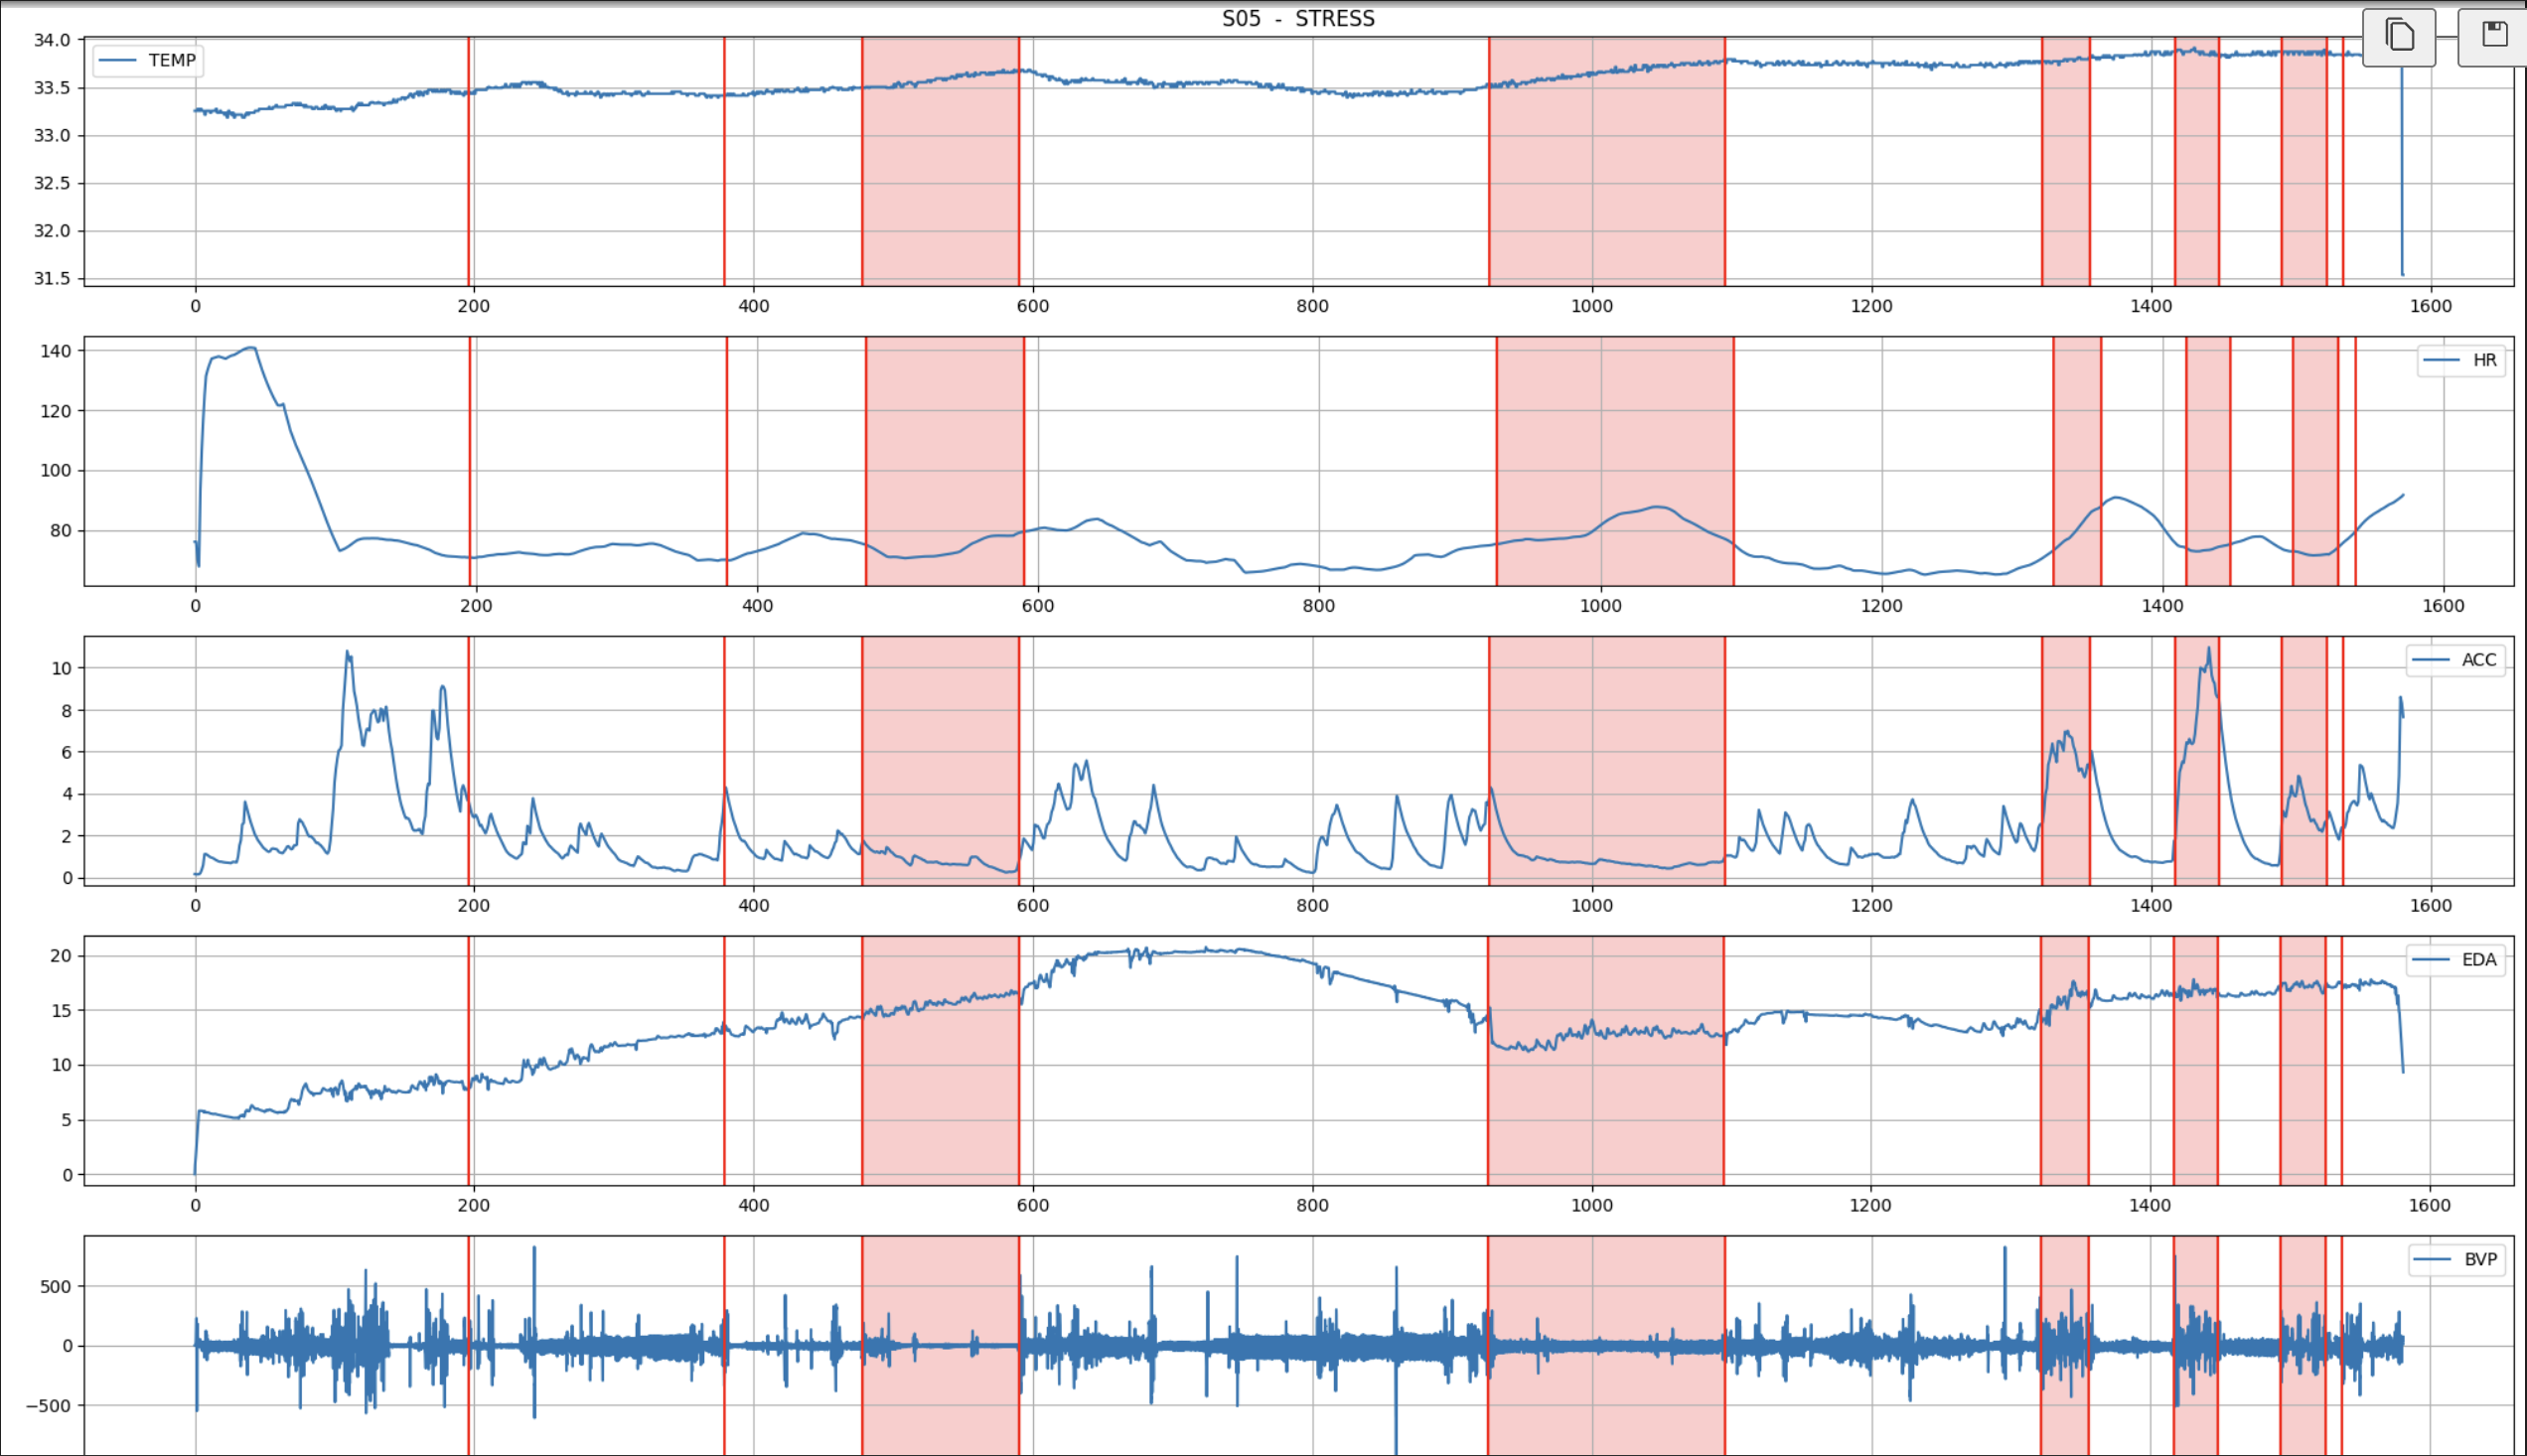
\includegraphics[width=1\linewidth]{S05_STRESS_signals.png}
    \caption{Physiological response signals for Subject S05 during the STRESS protocol. 
    Each subplot corresponds to one of the five recorded modalities (TEMP, HR, ACC, EDA, BVP). 
    Red-shaded intervals represent annotated stress-inducing periods where sympathetic activity is heightened. 
    Observable trends include an initial rise in skin temperature, sharp fluctuations in heart rate, and 
    increases in electrodermal activity concurrent with stress stimuli.}
    \label{fig:s05_stress_signals}
\end{figure}

\subsubsection{Physiological Signal Trends under Stress}
Figure~\ref{fig:s05_stress_signals} illustrates how multiple physiological modalities respond to mental stress induction.
Distinct patterns can be observed:
\begin{itemize}
    \item \textbf{Heart Rate (HR):} Rapid spikes followed by short recovery periods reflect acute autonomic arousal.
    \item \textbf{EDA:} Gradual increases in skin conductance correspond to sympathetic nervous activation.
    \item \textbf{ACC:} Low movement variance indicates minimal motion interference during the mental stress test.
    \item \textbf{TEMP \& BVP:} Show smoother upward trends suggesting vasodilation and thermoregulation responses.
\end{itemize}
Such multimodal profiles allow downstream classification models to learn discriminative stress signatures from raw sensor data.






\subsection{PMData description}
PMData is a multimodal personal logging dataset containing daily physiological and subjective wellness markers across 16 participants over a five month period. \citep{thambawita2020pmdata}.The dataset contains data from three sources: the Fitbit Versa 2 smartwatch provides biometric data, the PMSys sports logging app captures subjective wellness data, and Google forms collects demographic, food, and weight information. The Fitbit Versa 2 tracks physiological signals like heart rate, sleep patterns, and activity levels. The PMSys app allows participants to log daily metrics including stress, fatigue, mood, and readiness. Google Forms adds context through demographic information and lifestyle tracking. 

\begin{table}[H]
\centering
\renewcommand{\arraystretch}{1.2} 
\setlength{\tabcolsep}{6pt} 
\caption{Summary of PMData sources and number of entries.}
\label{tab:pmdata-summary}
\begin{tabular}{p{3.5cm}p{4cm}p{6.5cm}}
\toprule
\textbf{Source} & \textbf{Files / Reports} & \textbf{Examples of Data Collected} \\
\midrule
Fitbit Versa~2 & $\sim$21{,}000{,}000\,heart rate samples & Heart rate, sleep score, steps, calories, and time in heart rate zones. \\
PMSys App & 1{,}747\,wellness reports & Stress, fatigue, mood, readiness, sleep duration, and sleep quality. \\
Google Forms & 1{,}569\,daily entries & Weight, alcohol, water intake, and meals. \\
\bottomrule
\end{tabular}
\end{table}

Each particpant's folder contains Fitbit JSON files, PMSys CSV files, and google form data. All files include timestamps, which make it possible to align entries by date. 

\paragraph{Processing Steps.} We used the PMSys \texttt{wellness.csv} file to obtain our main target variable,the daily \texttt{stress} score (1--5 scale). 
Fitbit data, which is collected every minute, was summarized into daily averages 
and totals such as mean heart rate, total active minutes, and previous-night sleep score. We then merged Fitbit and PMSys data by participant and date to create a consistent daily dataset.

Fitbit data is collected at a high frequency, while PMSys stress ratings occur once a day. Aggregating Fitbit signals by day ensures that each stress label is paired 
with corresponding daily physiological data. This makes the datasets comparable and helps our model learn relationships between daily stress levels and overall physiological patterns.


\FloatBarrier
\begin{table}[htbp]
\centering
\renewcommand{\arraystretch}{1.2} % add vertical spacing
\setlength{\tabcolsep}{6pt}       % adjust horizontal padding
\caption{Relevant PMData columns used in the analysis.}
\label{tab:pmdata-cols}
\begin{tabular}{p{3.2cm}p{3.2cm}p{7.8cm}}
\toprule
\textbf{File} & \textbf{Column Name} & \textbf{Description / Use} \\
\midrule
\texttt{wellness.csv} & \texttt{stress} & Target variable (1--5 scale) of self-reported daily stress; used as ground truth. \\
                      & \texttt{sleep\_duration\_h} & Total hours of sleep reported each night. \\
                      & \texttt{sleep\_quality} & Subjective rating of sleep quality. \\[4pt]
\texttt{heart\_rate.json} & -- & Minute-level heart rate readings used to compute daily averages and variability. \\
\texttt{time\_in\_heart\_rate\_zones.json} & -- & Duration spent in heart-rate zones (fat burn, cardio, peak); indicator of intensity and stress response. \\
\texttt{resting\_heart\_rate.json} & -- & Daily resting heart rate; used to track baseline changes. \\
\texttt{sleep.json} & -- & Detailed sleep-phase data (light, deep, REM, awake). \\
\texttt{sleep\_score.csv} & -- & Overall sleep-quality score (0–100) summarizing duration, composition, and restfulness. \\
\bottomrule
\end{tabular}
\end{table}



\paragraph{Exploratory Data Analysis}
Basic exploration of PMData shows that:
\begin{itemize}
    \item Most stress ratings cluster around 2-3, suggesting mild to moderate stress on average.
    \item Participants with higher average heart rates also tend to report higher stress levels.
    \item Days with lower sleep quality often correspond to slightly higher stress and fatigue.
\end{itemize}

These observations support the idea that physiological patterns (heart rate and sleep) 
relate to subjective stress levels, making PMData suitable for modeling daily stress.

\begin{figure}[!ht]
\centering
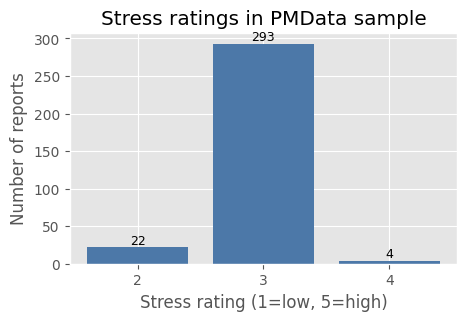
\includegraphics[width=0.5\linewidth]{Stress Distribution.png}
\caption{Distribution of self-reported stress ratings in the PMData sample.}
\label{fig:stress-dist}
\end{figure}

\begin{figure}[htbp]
\centering
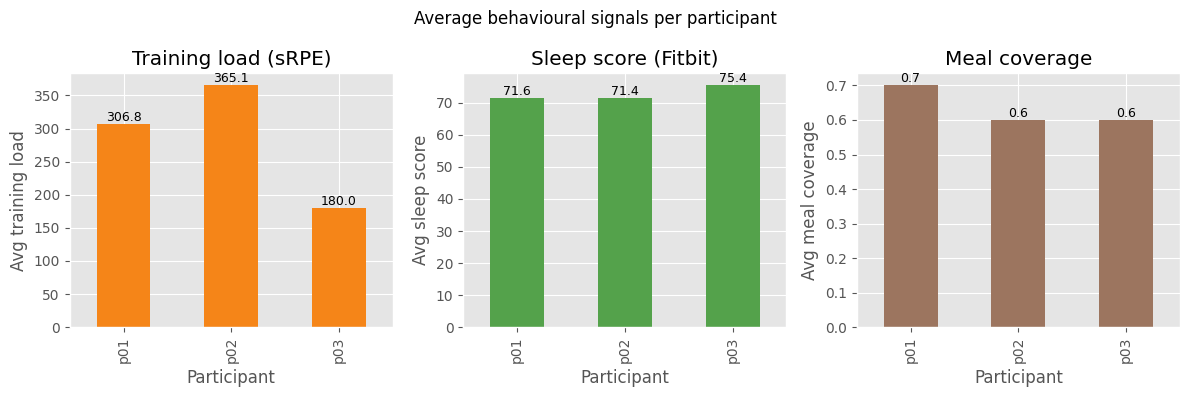
\includegraphics[width=0.85\linewidth]{Avg_BeHparticipant.png}
\caption{Average behavioral signals across three participants in the PMData sample. Training load measured by session Rating of Perceived Exertion (sRPE) from PMSys app.}
\label{fig:participant-metrics}
\end{figure}


\paragraph{Relevance to Our Study.}
This dataset will be used to bridge controlled stress induction data collected with the Empatica~E4 wearable and free-living, personalized lifelog data from PMData. By combining these two sources, we can test how stress patterns learned in lab settings transfer to real-world environments. PMData provides continuous wearable signals (heart rate, sleep, and activity) together with daily self-reported stress, which allows us to adapt and evaluate lab-trained stress models for practical, real-world use.


\paragraph{Limitations.}
\begin{itemize}
    \item Small sample size (16 participants) and some missing days.
    \item Stress and wellness ratings are self-reported and may be subjective.
    \item Fitbit data can include small measurement errors or gaps.
\end{itemize}
Despite these limitations, PMData offers realistic, noisy data that is valuable 
for studying stress detection in everyday settings.


%%%%%%%%%%%%%%%%%%%%%%%%%%%%%%%%%%%%%%%%%%%%%%%%%%%%%%%%
%%%% Reference / Bibliography
%%%%%%%%%%%%%%%%%%%%%%%%%%%%%%%%%%%%%%%%%%%%%%%%%%%%%%%%

\section*{References}

\noindent Schlink, B., and O. Amft. (2020). \textit{WISE: Wearable Stress and Exercise Dataset.} Scientific Reports, 10(1), 23010. Springer Nature. \\[4pt]
Schmidt, P., A. Reiss, R. Duerichen, C. Marberger, and K. Van Laerhoven. (2018). \textit{Introducing WESAD, a Multimodal Dataset for Wearable Stress and Affect Detection.} Proceedings of the 20th ACM International Conference on Multimodal Interaction (ICMI ’18). Association for Computing Machinery. \\[4pt]
Soto, D., F. Falcioni, and R. Damasio. (2021). \textit{Sports DB: A Multimodal Cardiorespiratory Dataset for Sports Activity Recognition.} Data in Brief, 36, 107116. Elsevier. \\[4pt]
Moore, J., T. C. Pataky, and J. P. Richards. (2020). \textit{BioCV: A Biomechanical Computer Vision Motion Capture Dataset for Human Movement Analysis.} University of Bath Motion Analysis Research Group. \\[4pt]
Zhao, M., and D. Maltoni. (2023). \textit{GLOBEM: Global Multi-Year Mobile and Wearable Sensing Dataset for Behavioral and Mental Health Modeling.} arXiv preprint arXiv:2211.02733. \\[4pt]
Hickey, B. A., et al. (2021). \textit{Smart Devices and Wearable Technologies to Detect and Monitor Mental Health Conditions and Stress: A Systematic Review.} Sensors, 21(10), 3461. MDPI. \\[4pt]
Thambawita, V., et al. (2020). \textit{PMData: A Sports Logging Dataset.} Proceedings of the 11th ACM Multimedia Systems Conference (MMSys ’20), Istanbul, Turkey, 231–236. Association for Computing Machinery.



% \bibliography{reference}
% \bibliographystyle{style/dsc180bibstyle}

%%%%%%%%%%%%%%%%%%%%%%%%%%%%%%%%%%%%%%%%%%%%%%%%%%%%%%%%
%%%% Appendix
%%%%%%%%%%%%%%%%%%%%%%%%%%%%%%%%%%%%%%%%%%%%%%%%%%%%%%%%

\clearpage
\makeappendix

\subsection{Training Details}

\subsection{Additional Figures}

\subsection{Additional Tables}


\end{document}


%%% STUFF FROM TEMPLATE BELOW: 
Here's \textbf{bold} and \textit{italicized} text. Here's \texttt{text\_that\_looks.like(code)}.

\begin{itemize}
    \item Here's a regular bulleted list item.
    \item And another.
\end{itemize}

Here's a \href{https://datascience.ucsd.edu}{hyperlink}. If you want to use a numbered list, you can experiment with:

\begin{enumerate}
    \item This.
    \item This.
    \item And this.
\end{enumerate}

Here's how you might include a snippet of actual code:

\begin{verbatim}
# If you want to use syntax highlighting, look into the minted package.
def f(x):
    return 2 * x + 3
\end{verbatim}

Here's how you might format a single equation:

$$\int_{-\infty}^\infty f_X(x)dx = 1$$

And a chain of equations:

\begin{align*}
    \frac{1}{n}\sum_{i = 1}^n (x_i - \bar{x})^2 &= \frac{1}{n}\sum_{i = 1}^n (x_i^2 - 2x_i\bar{x} + \bar{x}^2)
    \\ &= \frac{1}{n}\sum_{i = 1}^n x_i^2 - \frac{2}{n}\bar{x}\sum_{i = 1}^n x_i + \frac{\bar{x}^2}{n}\sum_{i = 1}^n 1
    \\ &= \frac{1}{n}\sum_{i = 1}^n x_i^2 - 2\bar{x}^2 + \bar{x}^2
    \\ &= \frac{1}{n}\sum_{i = 1}^n x_i^2 - \bar{x}^2
\end{align*}


\subsection{Figure Examples}

Here are some example figures. 
Figure \ref{fig:somefig1} presents a scatter plot.

\begin{figure}[htbp]
\centering
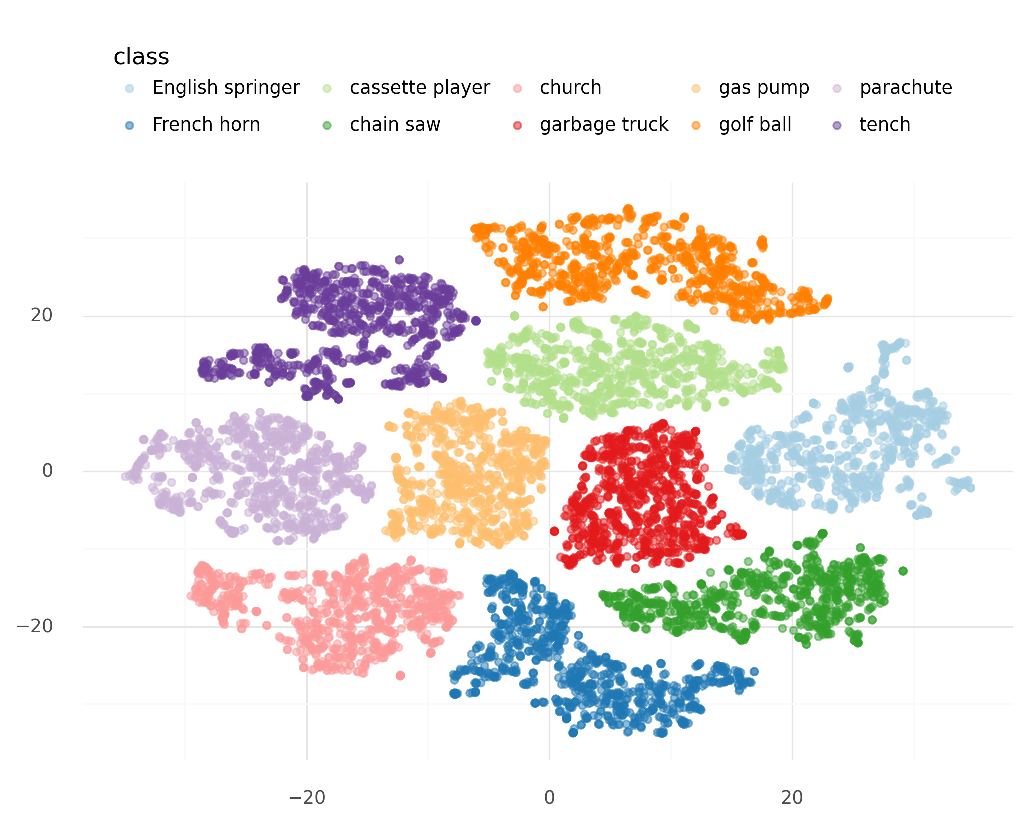
\includegraphics[width=.65\linewidth]{figure/somefig1.pdf}
\caption{Yes, put a few words or sentences here explaining what is in the figure.}
\label{fig:somefig1}
\end{figure}

Figure \ref{fig:someotherfigs} presents some summaries of the performance of our model.
The left panel of Figure \ref{fig:someotherfigs} presents something.
The right panel of Figure \ref{fig:someotherfigs} presents some other things.

\begin{figure}[htbp]
\begin{minipage}{0.53\linewidth}
  \centering
  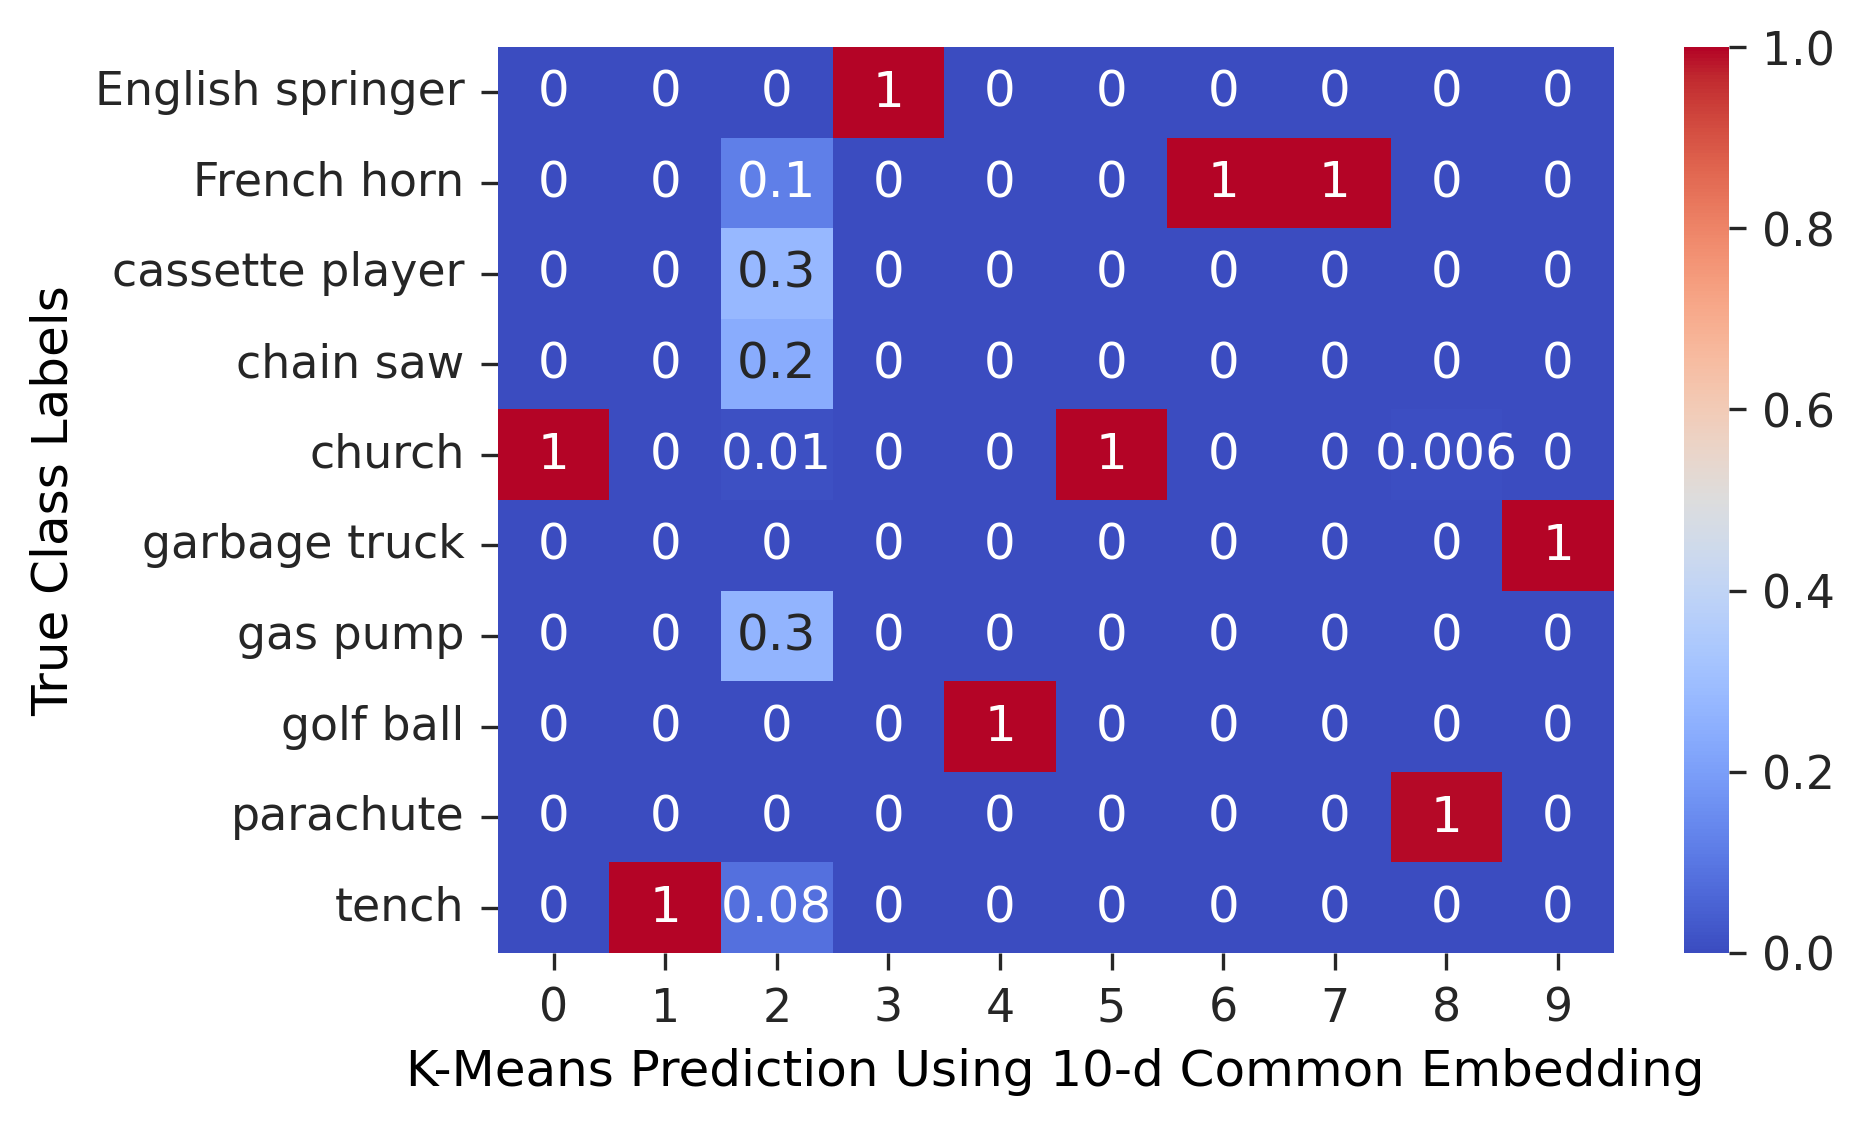
\includegraphics[width=\linewidth]{figure/somefig2.png}
\end{minipage}
\begin{minipage}{0.42\linewidth}
  \centering
  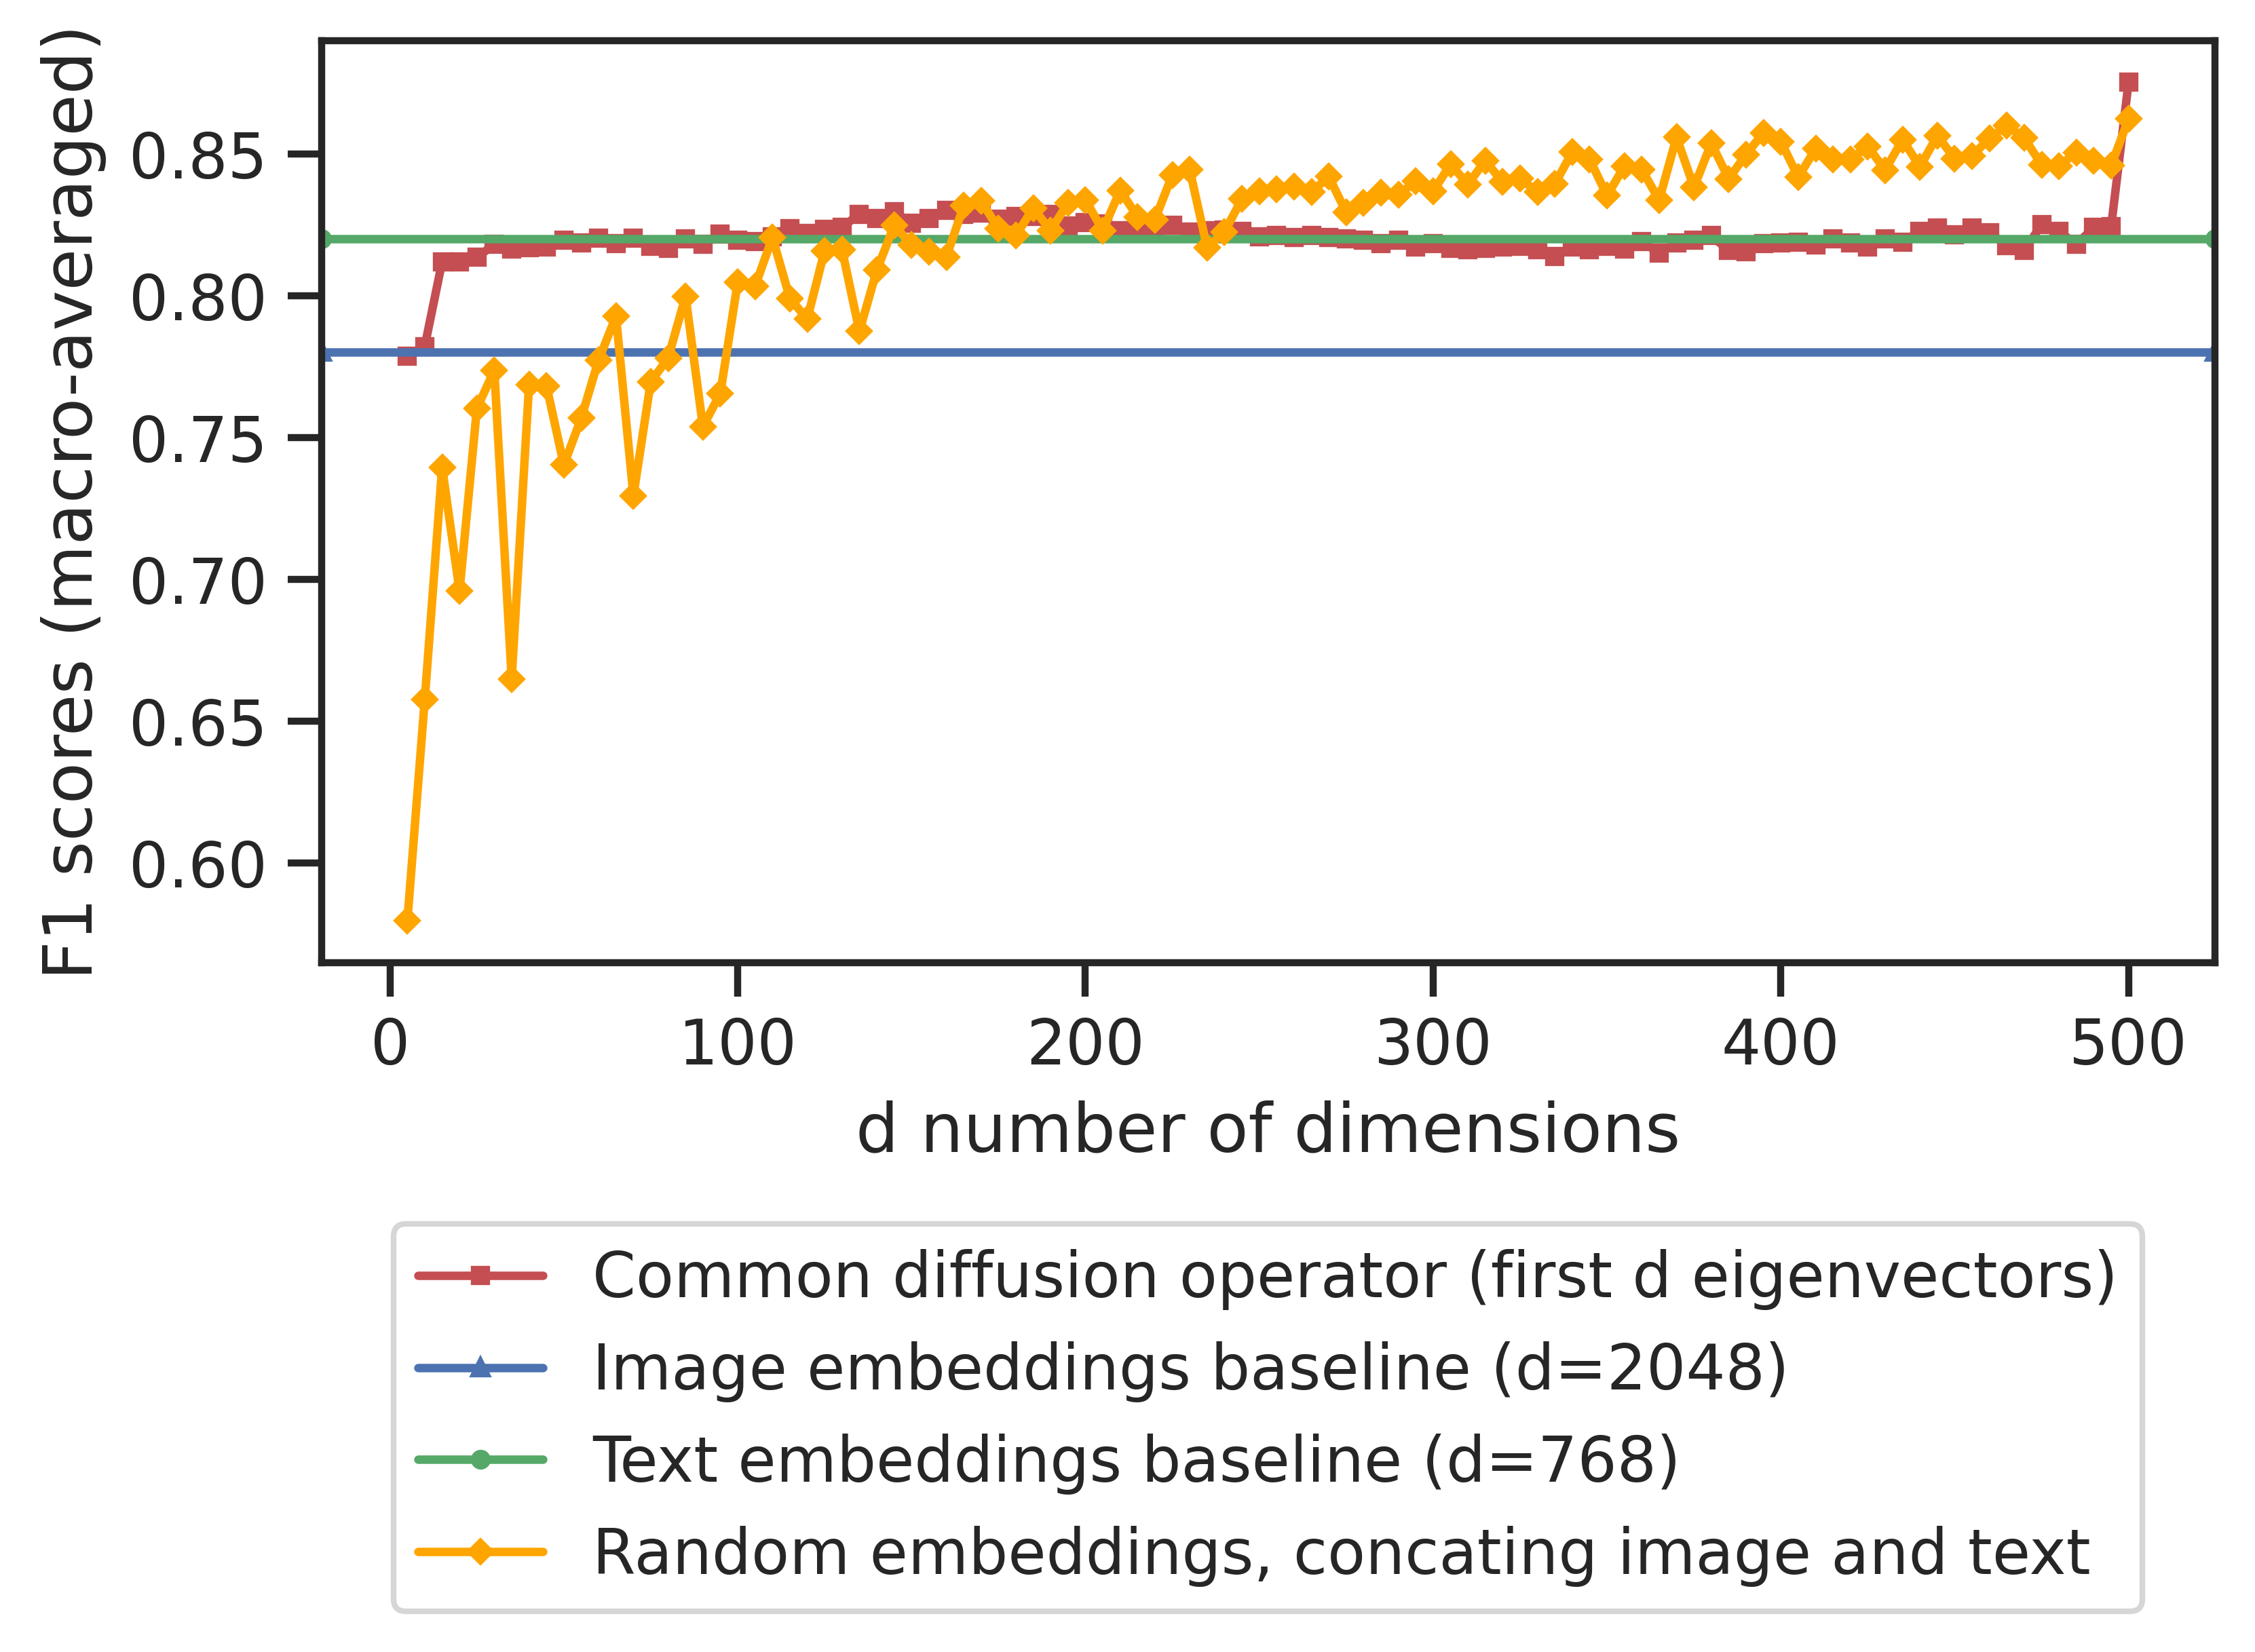
\includegraphics[width=\linewidth]{figure/somefig3.png}
\end{minipage}
\caption{You can put figures side-by-side as well.}
\label{fig:someotherfigs}
\end{figure}


\subsection{Table Examples}

Table \ref{tab:sometab1} presents some summary of the data.

\begin{table}[htbp]
\caption{Some Table Caption}
\label{tab:sometab1}
\resizebox{0.4\linewidth}{!}{\input{table/sometab1}}
\end{table}

Table \ref{tab:sometab2} presents some summaries of the performance of our model.

\begin{table}[htbp]
\caption{Some Other Table Caption}
\label{tab:sometab2}
\resizebox{0.9\linewidth}{!}{\input{table/sometab2}}
\end{table}

\subsection{Equations and Algorithms Examples}

Algorithm \ref{alg:fuzzyKmeans} implements Fuzzy K-means.

\begin{algorithm}
\caption{Fuzzy K-means clustering algorithm}
\label{alg:fuzzyKmeans}
\begin{enumerate}
    \item Choose primary centroids $v_{k}$
    \item Compute the membership degree of all feature vectors in all clusters
    \begin{equation}
    u_{ki}  = \frac{1}{ \sum_{j=1}^K ( \frac{D^{2}(x_{i} - v_{k})}{D^{2}(x_{i} - v_{j})})^\frac{2} 
    {m-1}}
    \label{eq:kmeans}
    \end{equation}
\end{enumerate}
\end{algorithm}

Algorithm \ref{alg:net} calculates net activation.


\begin{algorithm}
\caption{Computing Net Activation}
\label{alg:net}
% \DontPrintSemicolon
% \LinesNumbered
\KwIn{$x_1, \ldots, x_n, w_1, \ldots, w_n$}
\KwOut{$y$, the net activation}
$y\leftarrow 0$\;
\For{$i\leftarrow 1$ \KwTo $n$}{
$y \leftarrow y + w_i*x_i$\;
}
\end{algorithm}

In Variational Autoencoder (VAE), we directly maximize the Evidence Lower Bound (ELBO) using the following Equations \ref{eq:bla}--\ref{eq:blablabla}.
\begin{align}
  \mathbb{E}_{q_{\boldsymbol{\phi}}(\boldsymbol{z}\mid\boldsymbol{x})}\left[\log\frac{p(\boldsymbol{x}, \boldsymbol{z})}{q_{\boldsymbol{\phi}}(\boldsymbol{z}\mid\boldsymbol{x})}\right]
  &= \mathbb{E}_{q_{\boldsymbol{\phi}}(\boldsymbol{z}\mid\boldsymbol{x})}\left[\log\frac{p_{\boldsymbol{\theta}}(\boldsymbol{x}\mid\boldsymbol{z})p(\boldsymbol{z})}{q_{\boldsymbol{\phi}}(\boldsymbol{z}\mid\boldsymbol{x})}\right] \label{eq:bla} \\
  &= \mathbb{E}_{q_{\boldsymbol{\phi}}(\boldsymbol{z}\mid\boldsymbol{x})}\left[\log p_{\boldsymbol{\theta}}(\boldsymbol{x}\mid\boldsymbol{z})\right] + \mathbb{E}_{q_{\boldsymbol{\phi}}(\boldsymbol{z}\mid\boldsymbol{x})}\left[\log\frac{p(\boldsymbol{z})}{q_{\boldsymbol{\phi}}(\boldsymbol{z}\mid\boldsymbol{x})}\right] \label{eq:blabla} \\
  &= \underbrace{\mathbb{E}_{q_{\boldsymbol{\phi}}(\boldsymbol{z}\mid\boldsymbol{x})}\left[\log p_{\boldsymbol{\theta}}(\boldsymbol{x}\mid\boldsymbol{z})\right]}_\text{reconstruction term} - \underbrace{\mathcal{D}_{\text{KL}}(q_{\boldsymbol{\phi}}(\boldsymbol{z}\mid\boldsymbol{x}) \mid\mid p(\boldsymbol{z}))}_\text{prior matching term} \label{eq:blablabla}
\end{align}

\subsection{Inline Citation Examples}

Citation in text (no parentheses): use \texttt{{\textbackslash}cite\{citekey\}}. 
For example, \cite{breiman2011}, \cite{devlin2019bert}.

Citation in parentheses: use \texttt{{\textbackslash}citep\{citekey\}}. 
For example: \citep{vaswani2023attention}, \citep{karras2019stylebased}.



% \makereference

% {\color{blue} To edit the contents of the ``References" section, edit \texttt{reference.bib}. Many conference websites format citations in BibTeX that you can copy into \texttt{reference.bib} directly; you can also search for the paper on Google Scholar, click ``Cite", and then click ``BibTeX" (\href{https://scholar.google.com/scholar?hl=en&as_sdt=0%2C23&q=attention+is+all+you+need&btnG=#d=gs_cit&t=1700436667623&u=%2Fscholar%3Fq%3Dinfo%3A5Gohgn6QFikJ%3Ascholar.google.com%2F%26output%3Dcite%26scirp%3D0%26hl%3Den}{here}'s an example).}